\section*{Results and Discussion}

Starting with a simple TWFE estimate of the impact of additional off-menu expenditures, we conduct a discrete-choice analysis similar to that of \cite{berry1994}. 
Thus we conduct a simple logit model using off-menu expenditures (measured in \$ 100,00). 
This model results in the following simple regression results shown below, showing an increase in off-menu expenditures the year before an election matter and helps move the outcome towards the incumbent. 
If the results below were causal in the OLS case, this would mean that by spending the entire \$1.3M on off-menu projects, an alderperson could expect to increase their vote share from 30\% to 95\%. We further replicate the results with a direct beautification measure, which only counts public art and park spending.
 The results of substituting off-menu expenditures with beautification are shown in table 6 in the appendix. 
 Finally, the results were replicated with the 12 unopposed candidates, and the results were all statistically insignificant in that model. 
 These are shown in table 7 in the appendix.


\begin{table}[H] \centering 
  \caption{Impact of Off-Menu Expenditures with Binomial Choice, OLS, and with experience controls} 
  \label{} 
\begin{tabular}{@{\extracolsep{5pt}}lccc} 
\\[-1.8ex]\hline 
\hline \\[-1.8ex] 
 & \multicolumn{3}{c}{\textit{Model:}} \\ 
\cline{2-4} 
\\[-1.8ex] & Binomial Choice & OLS & Experience OLS\\ 
\\[-1.8ex] & (1) & (2)\\ 
\hline \\[-1.8ex] 
 off\_menu & 0.239$^{**}$ & 5.578$^{**}$ & 4.570$^{*}$ \\ 
  & (0.099) & (2.322) & (2.514) \\ 
  & & & \\ 
 exp &  &  & $-$0.377 \\ 
  &  &  & (0.363) \\ 
  & & & \\ 
 Constant & $-$0.855$^{*}$ & 30.163$^{**}$ & 35.830$^{**}$ \\ 
  & (0.497) & (11.593) & (12.799) \\ 
  & & & \\ 
\hline \\[-1.8ex] 
Observations & 71 & 71 & 71 \\ 
R$^{2}$ & 0.864 & 0.846 & 0.853 \\ 
Adjusted R$^{2}$ & 0.586 & 0.531 & 0.533 \\ 
Residual Std. Error & 0.328 (df = 23) & 7.651 (df = 23) & 7.639 (df = 22) \\ 
F Statistic & 3.107$^{***}$ (df = 47; 23) & 2.689$^{***}$ (df = 47; 23) & 2.664$^{***}$ (df = 48; 22) \\ 
\hline 
\hline \\[-1.8ex] 
\textit{Note:}  & \multicolumn{3}{r}{$^{*}$p$<$0.1; $^{**}$p$<$0.05; $^{***}$p$<$0.01} \\ 
\end{tabular} 
\end{table} 

The results of the regression discontinuity analysis are given below. 
For this we used 4 bandwidth specifications, a "full" bandwidth that uses the entire data-set, an Imbens-Kalyanaraman bandwidth \cite{IK_bandwidth}, a mean-square-error(MSE) optimal bandwidth derived by Calonico et al.
 \cite{CCF_MSE}, and a coverage-error-probability (CER) optimal bandwidth derived by Calonico et al \cite{CCF_CER}. 
 The results show a large and barely significant effect of an incumbent just winning the election, regardless of the bandwidth size. 
 This result indicates that when the incumbent barely wins an election, this causes off-menu expenditures to decrease by more than \$100,000 relative to wards where challengers just barely beat out incumbents if the assumptions of continuity and random assignment close to the cutoff hold. 
 These results, if they are to be trusted, perhaps show potential problems with our supposed electoral mechanism. 
 If an electoral competency mechanism drove these results, then the results should show that there is no significant difference between alderpeople who just barely won and lost the election. 
 This is because if the voters split evenly between the two candidates, then it must be the case that they have practically equivalent competence. 
 However, as we will see, these results are not as steady as the p-value may indicate. 

\begin{table}[H] \centering 
  \caption{Regression Discontinuity Results for a Variety of Bandwidths} 
  \label{} 
\small 
\begin{tabular}{lcccc} 
\\[-1.8ex]\hline 
\hline \\[-1.8ex] 
 & \multicolumn{4}{c}{\textit{Bandwidth Criterion:}} \\ 
\cline{2-5} 
\\
 & Full & IK & MSE & CER \\ 
\\[-1.8ex] & (1) & (2) & (3) & (4)\\ 
\hline \\[-1.8ex] 
 IW & $-$111,845$^{**}$ & $-$129,425$^{***}$ & $-$173,271$^{***}$ & $-$152,452$^{***}$ \\ 
  & (47,501) & (38,302) & (46,566) & (49,220) \\ 
  & & & & \\ 
 IVS & 919,463$^{*}$ & 1,551,752$^{**}$ & 1,679,313$^{*}$ & 1,863,734 \\ 
  & (545,557) & (624,376) & (849,169) & (1,181,661) \\ 
  & & & & \\ 
 IW:IVS & $-$839,454 & $-$1,564,804$^{**}$ & 38,509 & $-$1,378,414 \\ 
  & (549,719) & (671,145) & (1,129,667) & (1,484,783) \\ 
  & & & & \\ 
 Constant & 140,967$^{***}$ & 159,083$^{***}$ & 161,626$^{***}$ & 164,978$^{***}$ \\ 
  & (44,467) & (33,981) & (38,497) & (40,705) \\ 
  & & & & \\ 
\hline \\[-1.8ex] 
Observations & 123 & 69 & 49 & 45 \\ 
R$^{2}$ & 0 & 0 & 0 & 0 \\ 
Adjusted R$^{2}$ & 0 & 0 & 0 & 0 \\ 
Residual Std. Error & 117,476 (df = 119) & 81,839 (df = 65) & 89,492 (df = 45) & 87,740 (df = 41) \\ 
F Statistic & 2 (df = 3; 119) & 4$^{***}$ (df = 3; 65) & 5$^{***}$ (df = 3; 45) & 4$^{**}$ (df = 3; 41) \\ 
\hline 
\hline \\[-1.8ex] 
\textit{Note:}  & \multicolumn{4}{r}{$^{*}$p$<$0.1; $^{**}$p$<$0.05; $^{***}$p$<$0.01} \\ 
\end{tabular} 
\end{table} 

The visual results of the regression discontinuity analysis are given below. 
Note how neither of the two assumptions required for the validity of the regression discontinuity design seems to hold. 
Firstly, the result is driven mainly by a large grouping of zero values to the left of the cutoff, indicating a non-random assignment. 
Secondly, there seems to be a significant increase in density right after the cutoff, indicating sorting issues. 
Finally, the data seems incredibly dispersed and can hardly be considered continuous. 

\begin{figure}[H]
    \centering
    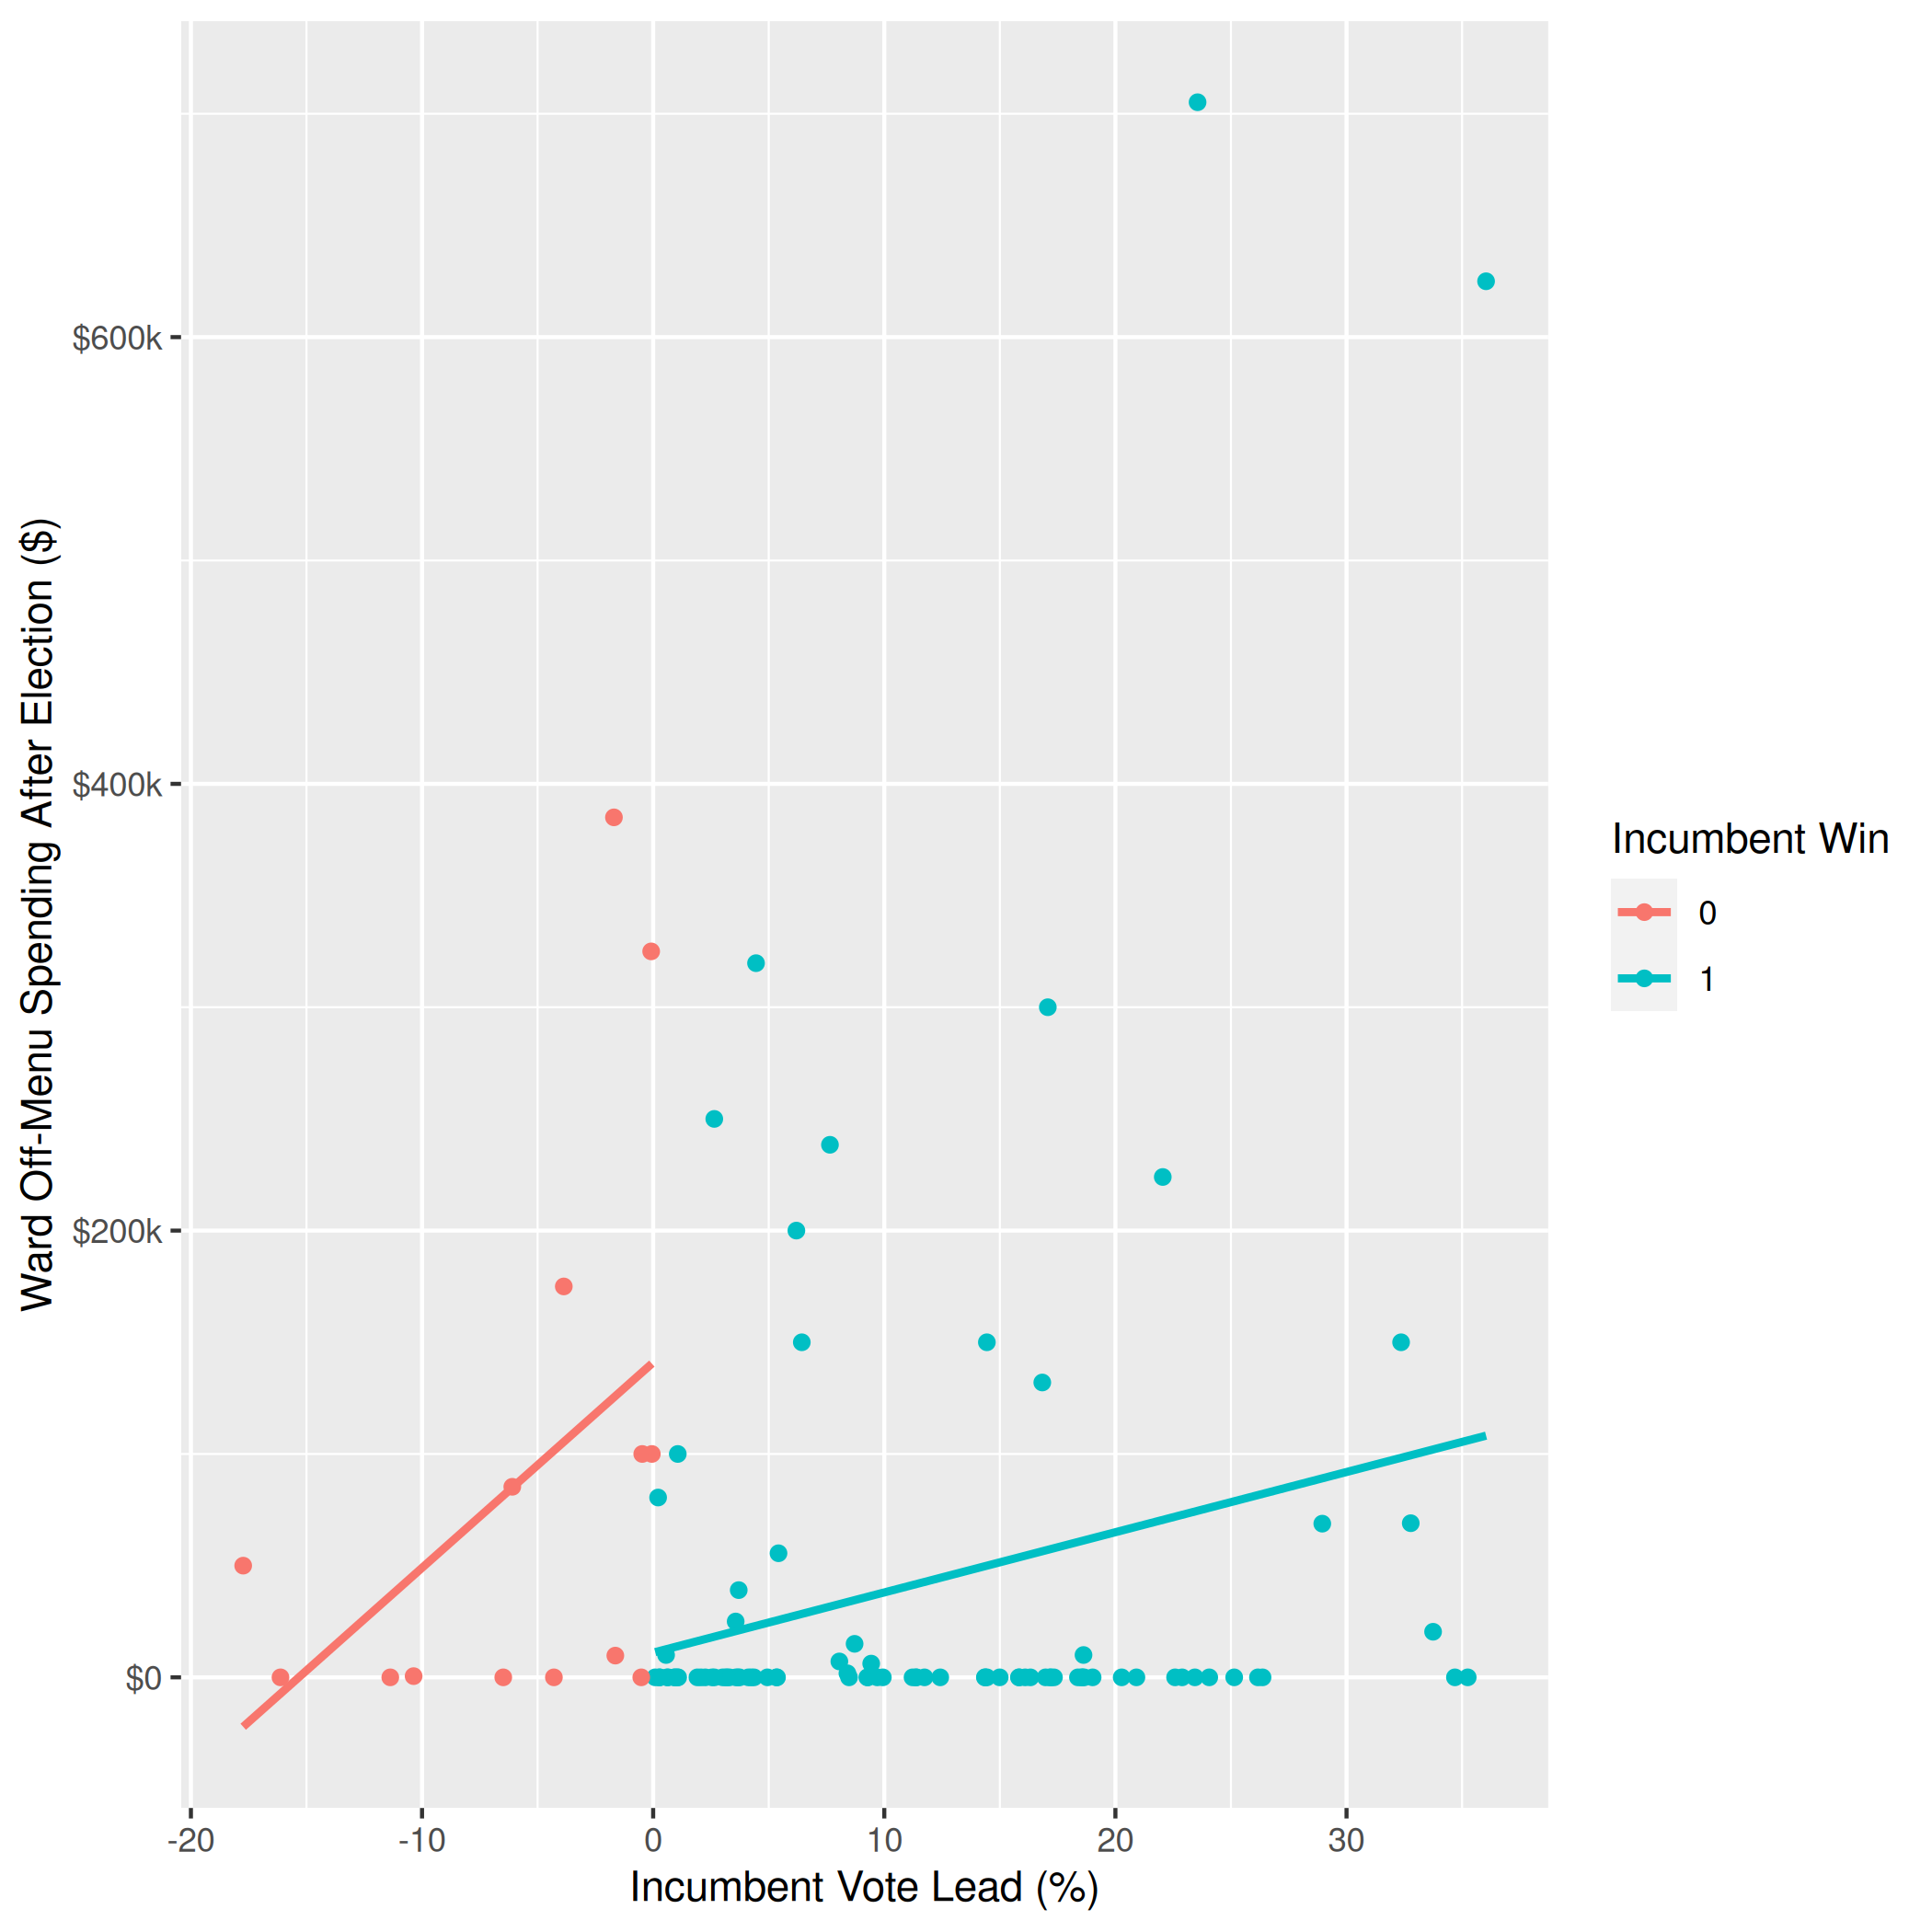
\includegraphics[scale=0.8]{input/RDD_plot.png}
        \caption{RDD results across 2011, 2015, and 2019 elections on off-menu expenditures}
\end{figure}

To verify the integrity of the regression discontinuity analysis, we perform two diagnostic procedures: A Mccrary-density test and a placebo test \cite{MCCRARY2008698}. 
The Mccrary-density test is intended to verify the random-assignment assumption, and the placebo test is intended to verify the continuity assumption. 
Starting with the Mccrary density test, we see that the visual intuition was correct. 
There is a large and statistically significant discontinuity in data density at the cutoff. 
The P-Value generated from the McCrary test is 0.00354, well below the 0.05 significance level. 
This result may be from retirement selection or the endorsement-selection reasons discussed in the methodology section. 
However, regardless of the reason for the gap, this is a significant indication that the regression discontinuity analysis is flawed.

\begin{figure}[H]
    \centering
    \includegraphics[scale=0.7]{input/rdd_densityplot.png}
    \caption{Mccrary Density Test Plot}
\end{figure}

Next, we conducted a placebo test on the right side of the cutoff (due to a lack of examples of the challenger winning on the left side of the cutoff). 
We find that estimated effects range from being staunchly positive to highly negative as we move further away from the cutoff. 
However, out of 20 placebo tests, 5 achieve statistically significant levels, which is deeply concerning as it may indicate that the data generating process is inherently discontinuous, so the assumption of continuity concerning the running variable may be violated. 

\begin{figure}[H]
    \centering
    \includegraphics[scale=0.8]{input/RD_placebo_estimate.png}
    \includegraphics[scale=0.8]{input/RD_placebo_pvalue.png}
    \caption{Placebo Test Results}
\end{figure}

Now moving towards diff-in-diff analysis, we show the development of the treated and non-treated wards, where treated wards are the 12 wards where the previous alderman either was elected out of the office or retired in 2015. 
From the plot, off-menu expenditures track between both groups closely prior to 2016 and then take a significant increase. 
Note that alderpersons typically take over control of the menu fund the year after they get elected \cite{particpatory_budgeting_scrapping} since they asked to approve the budget of their predecessor. 
Thus, this plot can be seen as profoundly consistent with the concept that newer alderpersons tend to spend more on off-menu expenditures. 


\begin{figure}[H]
    \centering
    \includegraphics[scale=0.8]{input/did_plot.png}
    \caption{Line plot of Off-menu expenditures}
\end{figure}

The results of the simple TWFE DiD analysis are given below in table 5. 
We include three specifications, one that uses all data and treats retiring alderpersons and council members elected out of office equally, and one reduced specification for each treatment. 
$treated_1$ is the dummy variable indicating that a group is in the post-period of 2016 on-wards and is in the treatment group. 
Each subsequent $treated$ variable estimates the effect in the post-period, so $treated_2$ is the estimate for the 2017 period, and so on. 
The 50 data points from 2020 are excluded due to the 2019 election. 

% Table created by stargazer v.5.2.3 by Marek Hlavac, Social Policy Institute. E-mail: marek.hlavac at gmail.com
% Date and time: Tue, Jun 21, 2022 - 04:53:19 PM
\begin{table}[H] \centering 
  \caption{TWFE DiD specification} 
  \label{} 
\begin{tabular}{@{\extracolsep{5pt}}lccc} 
\\[-1.8ex]\hline 
\hline \\[-1.8ex] 
 & \multicolumn{3}{c}{\textit{Dependent variable:}} \\ 
\cline{2-4} 
\\[-1.8ex] & \multicolumn{3}{c}{off menu expenditures} \\ 
\\[-1.8ex] & Both & Elected Only & Retired Only\\ 
\hline \\[-1.8ex] 
 treated\_1 & 116,597.900$^{***}$ & 98,598.880$^{**}$ & 87,257.720 \\ 
  & (37,476.320) & (48,054.550) & (54,096.760) \\ 
  & & & \\ 
 treated\_2 & 76,880.010$^{**}$ & 27,719.370 & 41,346.880 \\ 
  & (37,476.320) & (48,054.550) & (54,096.760) \\ 
  & & & \\ 
 treated\_3 & 46,261.560 & 11,758.780 & 39,047.440 \\ 
  & (37,476.320) & (48,054.550) & (54,096.760) \\ 
  & & & \\ 
 treated\_4 & 22,180.280 & $-$60,015.080 & 47,998.510 \\ 
  & (37,476.320) & (48,054.550) & (54,096.760) \\ 
  & & & \\ 
 Constant & 401,848.100$^{***}$ & 51,387.300$^{**}$ & 401,106.800$^{***}$ \\ 
  & (38,318.320) & (22,857.340) & (38,839.330) \\ 
  & & & \\ 
\hline \\[-1.8ex] 
Observations & 400 & 360 & 328 \\ 
R$^{2}$ & 0.432 & 0.029 & 0.455 \\ 
Adjusted R$^{2}$ & 0.331 & $-$0.005 & 0.354 \\ 
Residual Std. Error & 101,227.700 (df = 339) & 128,918.500 (df = 347) & 101,381.900 (df = 276) \\ 
F Statistic & 4.296$^{***}$ (df = 60; 339) & 0.849 (df = 12; 347) & 4.511$^{***}$ (df = 51; 276) \\ 
\hline 
\hline \\[-1.8ex] 
\textit{Note:}  & \multicolumn{3}{r}{$^{*}$p$<$0.1; $^{**}$p$<$0.05; $^{***}$p$<$0.01} \\ 
\end{tabular} 
\end{table} 
The ATT(g,t) analysis results are depicted below, only for the full specification, including both treatments as equal. 
When the incumbent lost control of the fund in 2016, we observed a large increase in off-menu expenditures that is barely statistically significant at a level just above \$100,000, which is similar to the results shown in the discontinuity analysis and the simple TWFE analysis above. 
Furthermore, we tested parallel pre-trends using the event study framework discussed in \cite{CALLAWAY2021200} and found that we could not reject the null hypothesis of parallel pre-trends with a p-value of 0.7754. 

\begin{figure}[H]
    \centering
    \includegraphics[scale=0.8]{input/did_treatmenteffect_plot.png}
    \caption{Treatment effect plot}
\end{figure}


However, the figure above shows that the spike is largest after the election, and then the effect dies off before the next election. This effect is not what one would expect if the DiD estimator captured an electoral effect. 
If this were an electoral effect, we would most likely see the increase in off-menu expenditures happening right before the next election in 2018. However, that is not what we see. 
Thus, this is more likely some voter-selection effect. 
We looked into the 12 candidates who made up our treatment group and the primary issues in their campaigns. 
I found articles where four candidates cited public participation and presence as key themes of their campaign \, cite{wttw. 2015} \cite{dna.2015_18} \cite{dna.2015_35} \cite{dna.2015_7}. 
Thus, from this informal evidence and the data presented, the effect is more likely from the selection or the informational mechanisms and is unlikely to be the electoral mechanism. 